\section{\label{sec:selection}Event selection}
The event selection described in \cite{duet} used the PIA$\nu$o detector to identify events with no $\pi^{+}$ in the final state which are consistent with ABS+CX final states. For the analysis presented in this paper the selection was extended by using information from the downstream detector CEMBALOS to identify photons following a CX interaction. 

An illustration of a CX event is shown in Fig. \ref{fig:ev_disp}. The upstream horizontal (red) track is pion interacting in the PIA$\nu$O detector. Two photon trajectories (blue) are created from the decay of the $\pi^0$. One of those travels to CEMBALOS where it deposits charge as it converts. The other track (black) is a proton being ejected from the nucleus.

\begin{figure}[ht]
    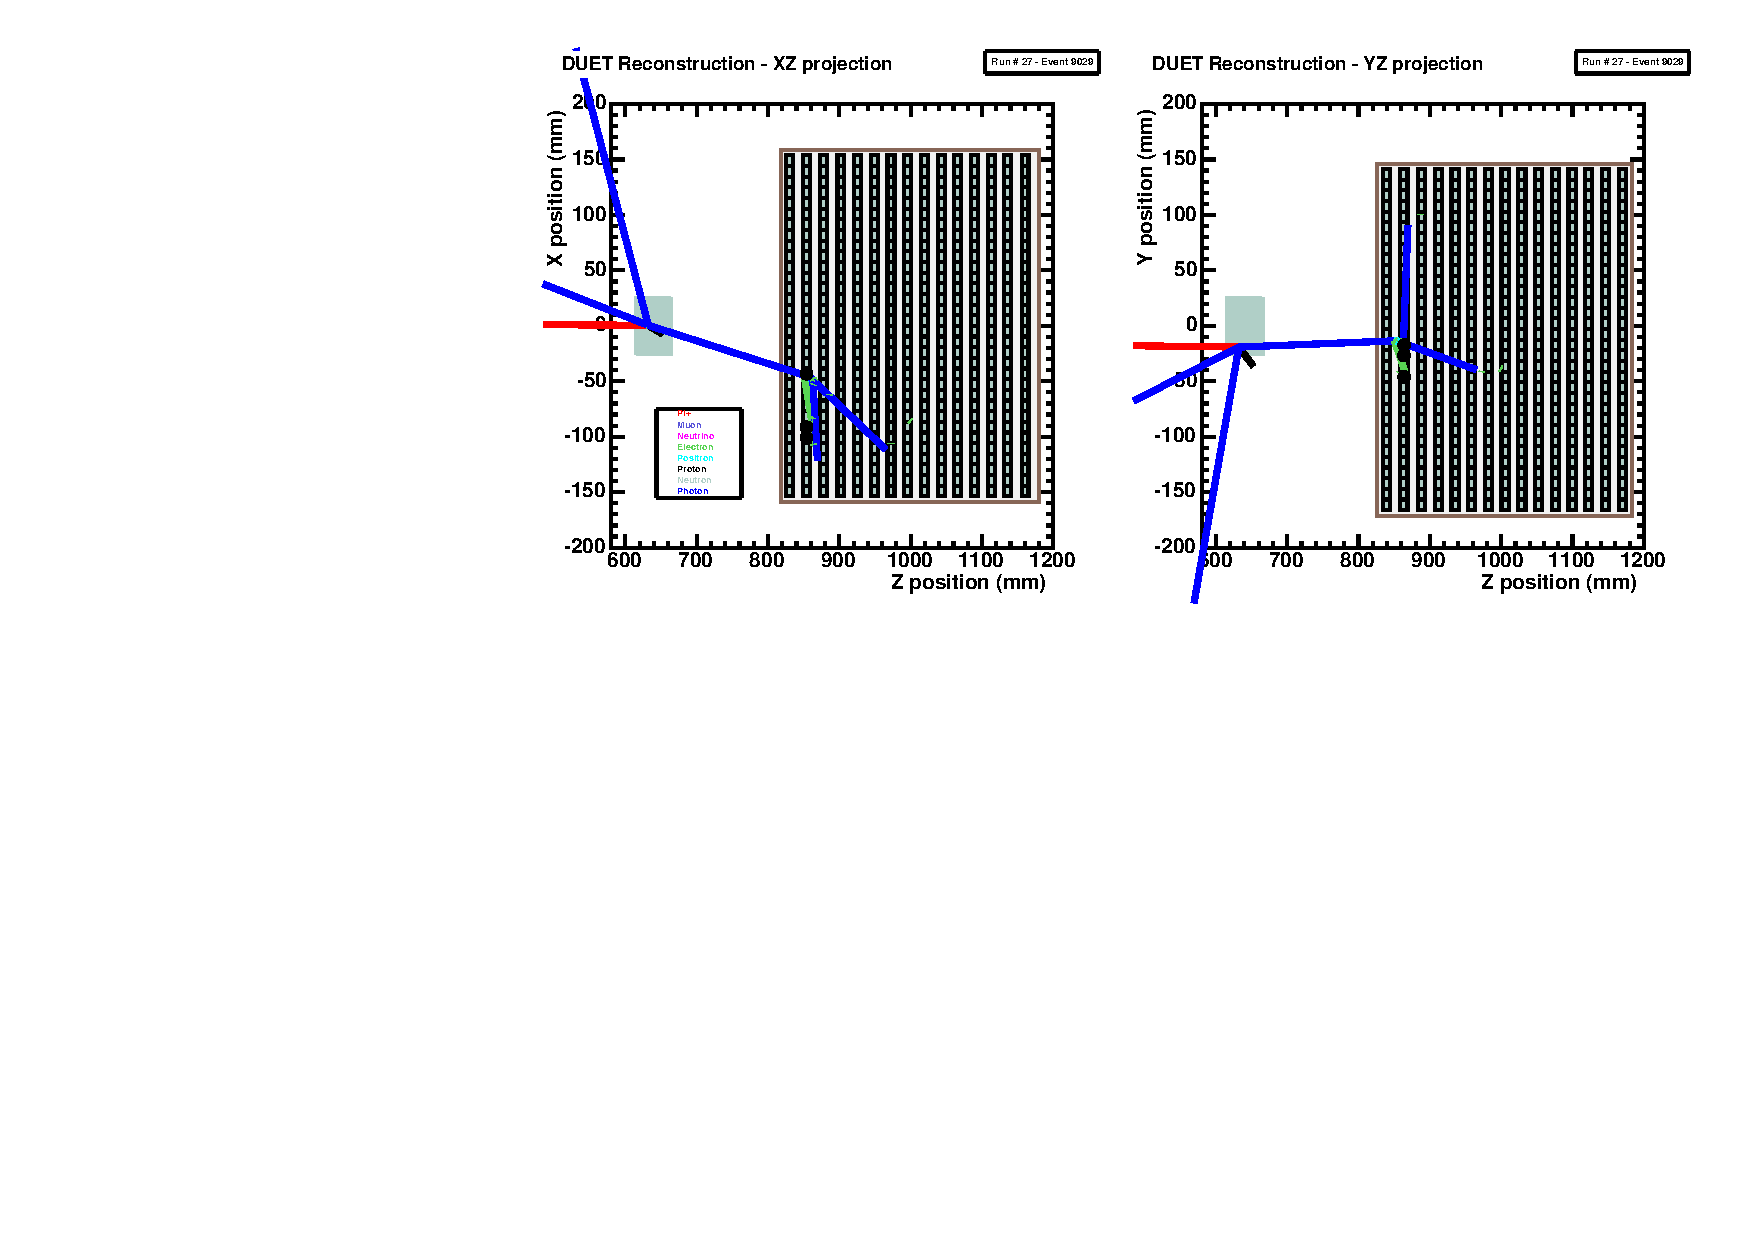
\includegraphics[width=90mm]{figures/ev_display_27_9029_intr4_ntag267.pdf}
    \caption{Example of a CX event ($p_\pi=$237.2 MeV$/c$). A $\pi^+$ (red) undergoes CX in PIA$\nu$O resulting in a $\pi^0$ decay to two photons (blue). A forward-going photon is identified in CEMBALOS as it showers and hits are recorded in the scintillating material.}
    \label{fig:ev_disp}
\end{figure}

\subsection{PIA$\nu$O upstream selection}
The PIA$\nu$O detector track reconstruction algorithm used charge deposition information to reconstruct and identify charged particles in the detector and to identify an interaction vertex. A detail description can be found in section III of \cite{duet}. A quick summary of the upstream selection criteria follows:
\begin{enumerate}
\item {\bf Good incident $\pi^{+}$\\}
This selection criteria is threefold: First, an incident $\pi^{+}$ was selected using TOF and Cherenkov light information. Second, a straight track, normal to the incident plane, leaving hits in the first 5 layers was required. Third, this incident track was required to enter a defined fiducial volume (FV).
\item {\bf Vertex inside the FV\\}
Events with pion interactions were selected by requiring a reconstructed vertex inside the FV. This removed through-going and pion events, as well as small-angle scattering events.
\item {\bf No $\pi^{+}$ final track\\}
Reconstructed tracks exiting the interaction vertex were classified into ``proton-like'' and ``pion-like" tracks using an angle-dependent cut on the deposited charge, $dQ/dx$. Events with no ``pion-like'' tracks in the final state were selected.
\end{enumerate}
There were $\sim$7000 selected events in data after these criteria was applied with a $\sim$79\% efficiency to select ABS+CX events occurring inside the FV. The purity was estimated to be $\sim$73\%. The main background were $\pi^{+}$ elastic and quasi-elastic scatterings. This selection was used to extract $\sigma{_\mathrm{ABS+CX}}$ in \cite{duet}.

\subsection{CEMBALOS selection}
Charge deposition information from CEMABALOS was used to identify CX interactions occurring in PIA$\nu$O. The main goal was to tag one of the photons produced by the decay of a $\pi^0$. The limited angular coverage ($\sim0.53 sr$) of CEMBALOS imposed the largest efficiency loss. The selection criteria was as follows:
\begin{enumerate}
\item{\bf Veto cut\\}
When charged particles arrived to CEMBALOS they immediately left a signal in the scintillator material. Figure \ref{fig:veto} shows the distribution of the position of the most upstream hit in CEMBALOS for each event. Each bar represents an XY module. A veto cut on the first two modules was applied to remove most of the charged background, such as as low-angle $\pi^+$ scatters and protons from ABS events.

\begin{figure}[ht]
 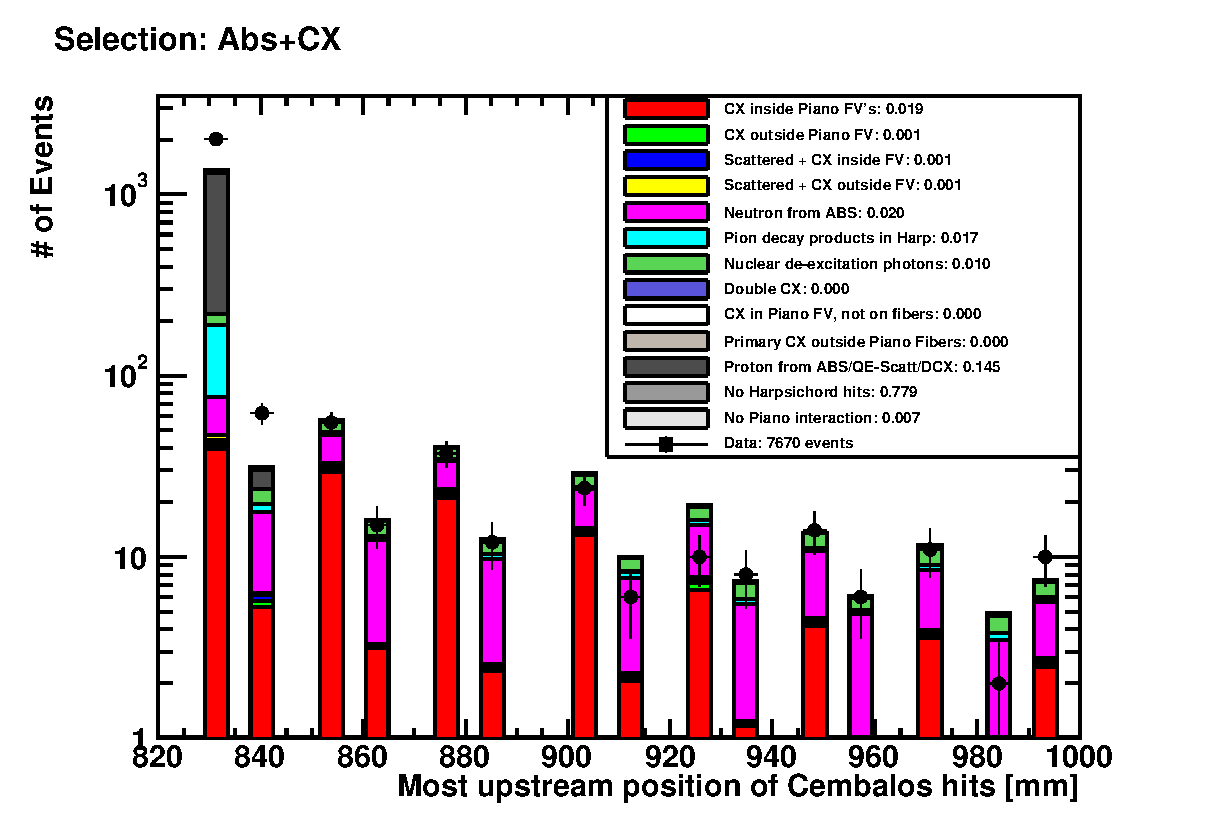
\includegraphics[width=86mm]{figures/duettag_fgdMostUp_10000.eps}
 \caption{(Color online) Distribution of the most upstream position of CEMABLOS hits for Data and MC in the $p_\pi=$237.2 MeV$/c$ setting after applying the PIA$\nu$O upstream selection. Each bar represents an XY module.}
 \label{fig:veto}
\end{figure}
   
\item{\bf Hit Charge vs. Multiplicity\\}
Neutrons from ABS events and nuclear de-excitation photons also mostly produced hits after the first two modules. Fig. \ref{fig:nhits} shows the distribution of the number of hits (multiplicity) in CEMBALOS. A minimum of 5 hits were required. Fig. \ref{fig:nhitsvsCharge} shows the CEMBALOS hit charge vs. multiplicity distribution after applying the previous requirement. A diagonal cut in this plane was applied to remove the remaining background of neutrons from ABS.
\end{enumerate}

\begin{figure}[ht]
 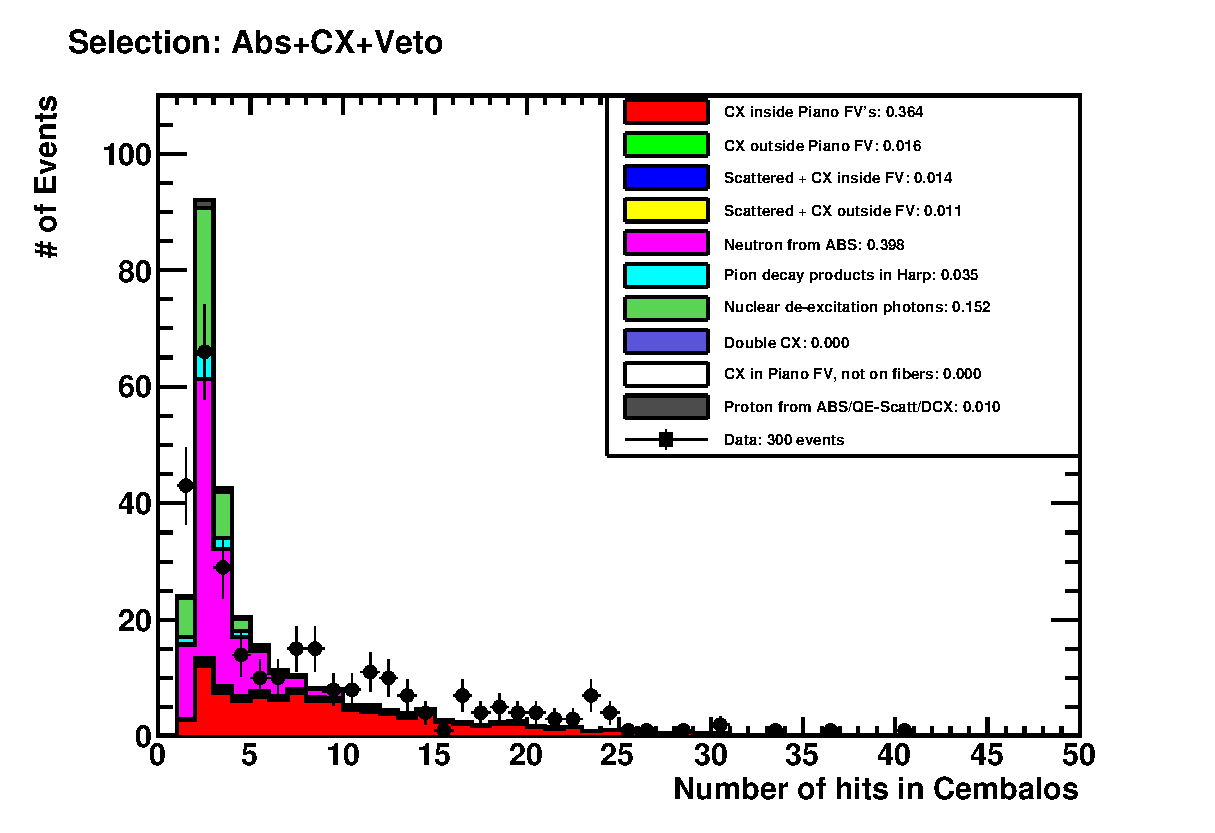
\includegraphics[width=86mm]{figures/duettag_nhits_20000.eps}
 \caption{(Color online) Distribution of the number of hits in CEMABLOS for Data and MC in the $p_\pi=$237.2 MeV$/c$ setting after applying the veto cut.}
 \label{fig:nhits}
\end{figure}

\begin{figure}[ht]
 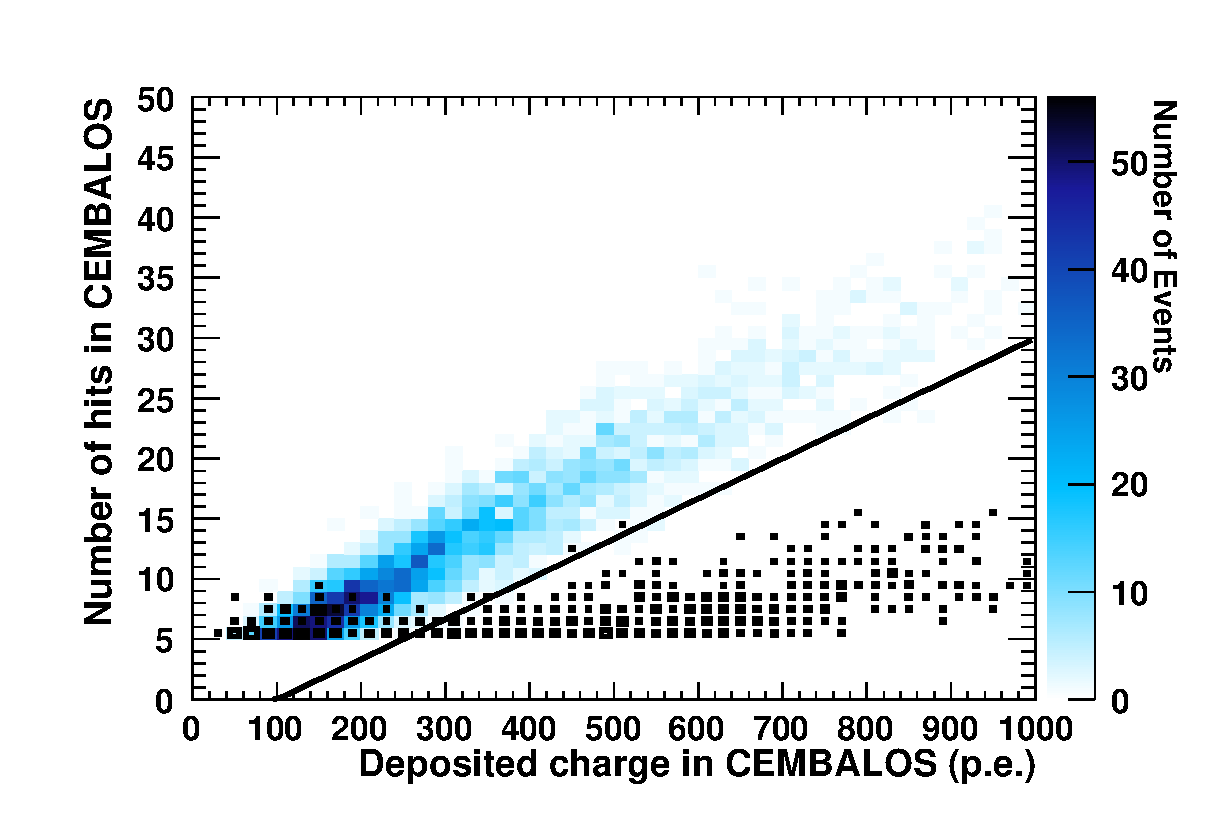
\includegraphics[width=86mm]{figures/draw2Dcut_draw.eps}
 \caption{(Color online) Distribution of the number of hits in CEMABLOS vs. charge deposited for Data and MC in the $p_\pi=$237.2 MeV$/c$ setting after applying the requirement of a minimum of 5 hits. The blue entries are true CX events, whereas the black boxes correspond to neutron background events.}
 \label{fig:nhitsvsCharge}
\end{figure}


\subsection{Selection purities and efficiencies}
The numbers of selected events for each momentum setting after the upstream and downstream selections were applied are summarized in Table \ref{tbl:short_event_summary} for data $N_{\mathrm{Data}}$ and MC (broken into signal $N_{\mathrm{CX}}^{\mathrm{MC}}$ and background $N_{\mathrm{BG}}^{\mathrm{MC}})$. There are $\sim$100 events in data after the event selection, with the exception of the 216.6 MeV$/c$ setting. The efficiencies and purities to select CX events which occurred inside the fiducial volume were around $\sim6\%$ and $\sim90\%$ respectively.

\begin{table}[h]
   \begin{tabular}{c|ccccc}
    \noalign{\hrule height 1pt}
    $p_{\pi}$  [MeV$/c$] & $N_{\mathrm{Data}}$ & $N_{\mathrm{CX}}^{\mathrm{MC}}$ & $N_{\mathrm{BG}}^{\mathrm{MC}}$ & Efficiency [\%] & Purity [\%] \\\hline
    201.6 & 104 & 60.4 & 8.6 & 5.1 & 87.5  \\
    216.6 & 20  & 15.8 & 2.4 & 5.3 & 86.6  \\
    237.2 & 141 & 75.9 & 11.1 & 5.9 & 87.2  \\
    265.6 & 152 & 87.1 & 10.4 & 7.0 & 89.3  \\
    295.1 & 163 & 119.4 & 12.8 & 8.1 & 90.3  \\
    \noalign{\hrule height 1pt}
   \end{tabular}
\caption{Summary of number of events selected after the CEMBALOS downstream selection in Data and MC for each momentum setting, along with estimated efficiencies and purities.}
\label{tbl:short_event_summary}
\end{table}

\section{$\sigma_{\mathrm{CX}}$ and $\sigma_{\mathrm{ABS}}$ extraction}\label{sec:xsec}
After the event selection described above, $\sigma_{\mathrm{CX}}$ is obtained in a similar fashion as in \cite{duet}. Corrections for the fraction of muons in the beam ($f_{\mu}$) and the fraction of interactions on nuclei other than Carbon ($R_{\mathrm{TiO}}^{\mathrm{Data}}$ and $R_{\mathrm{TiO}}^{\mathrm{MC}}$) were applied as shown in (\ref{eqn:xsec_calc}).

 \begin{equation} \label{eqn:xsec_calc}
 \begin{aligned}
 \sigma_{\mathrm{CX}} &= 
 \sigma_{\mathrm{CX}}^{\mathrm{MC}}
 \times \frac{N_{\mathrm{Data}}-N_{\mathrm{BG}}^{\mathrm{MC}}}{N_{\mathrm{CX}}^{\mathrm{MC}}} \\
 &\times
 \frac{1-R_{\mathrm{TiO}}^{\mathrm{Data}}}{1-R_{\mathrm{TiO}}^{\mathrm{MC}}}
 \times \frac{1}{1-f_{\mu}}
 \end{aligned}
 \end{equation} 
 
Where $\sigma_{\mathrm{CX}}^{\mathrm{MC}}$ is the CX cross section predicted by the Bertini cascade model in \textsc{Geant4}. $\sigma_{\mathrm{ABS}}$ is obtained by subtracting $\sigma_{\mathrm{CX}}$ from $\sigma_{\mathrm{ABS+CX}}$ from \cite{duet}.
 